\subsection{(10\%) Rasterization (2017 No. 8)}
Three vertices of a triangle have been sent through the OpenGL pipeline. 

They each have an (x, y) pixel position as well as a varying color value \textbf{c}.

\begin{enumerate}
    \item[P1:] position=( 5,  7), c= 0.4
    \item[P2:] position=(17, 27), c= 0.0
    \item[P3:] position=(11, 37), c= 1.0
\end{enumerate}

\subsubsection{What will the fragment shader value of \textbf{c} be set to at pixel (12, 22)?}

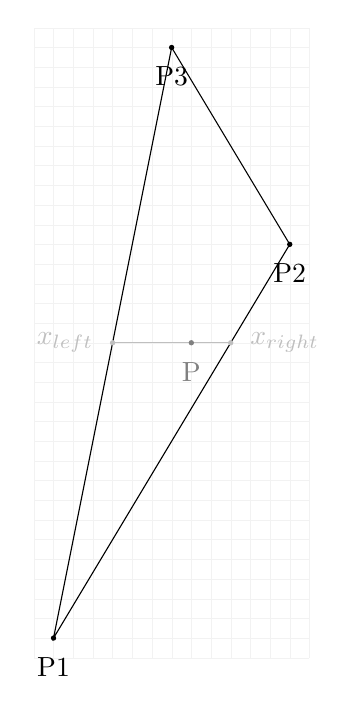
\begin{tikzpicture}[scale=0.25]
    \draw[step=1.0cm, gray!10, ultra thin](4, 6) grid (18, 38);
    \coordinate (P1) at ( 5,  7);
    \coordinate (P2) at (17, 27);
    \coordinate (P3) at (11, 37);
    \coordinate (xl) at (8, 22);
    \coordinate (xr) at (14, 22);
    \coordinate (P)  at (12, 22);
    
    \draw (P1) -- (P2) -- (P3) -- cycle;
    \draw[gray!50] (xl) -- (xr);
    
    \filldraw (P1) circle (3pt) node[label={below:P1}] {};
    \filldraw (P2) circle (3pt) node[label={below:P2}] {};
    \filldraw (P3) circle (3pt) node[label={below:P3}] {};
    \filldraw[gray!50] (xl) circle (3pt) node[label={left:$x_{left}$}] {};
    \filldraw[gray!50] (xr) circle (3pt) node[label={right:$x_{right}$}] {};
    \filldraw[gray] (P)  circle (3pt) node[label={below:P}] {};
\end{tikzpicture}

$y_{bot} = 7$

$y_{top} = 37$

$
    x_{left}
=
    lerp\left(P1.x, P3.x, \frac{y - P1.y}{P3.y - P1.y}\right)
=
    lerp\left(5, 11, \frac{22 - 7}{37 - 7}\right)
=
    8
$

$
    x_{right}
=
    lerp\left(P1.x, P2.x, \frac{y - P1.y}{P2.y - P1.y}\right)
=
    lerp\left(5, 17, \frac{22 - 7}{27 - 7}\right)
=
    14
$

$
    c_{left}
=
    lerp\left(P1.c, P3.c, \frac{y - P1.y}{P3.y - P1.y}\right)
=
    lerp\left(0.4, 1.0, \frac{1}{2}\right)
=
    0.7
$

$
    c_{right}
=
    lerp\left(P1.c, P2.c, \frac{y - P1.y}{P2.y - P1.y}\right)
=
    lerp\left(0.4, 0.0, \frac{3}{4}\right)
=
    0.1
$

$
    c_{pixel}
=
    lerp\left(c_{left}, c_{right}, \frac{P.x - x_{left}}{x_{right} - x_{left}}\right)
=
    lerp\left(0.7, 0.1, \frac{12 - 8}{14 - 8}\right)
=
    0.3
$

The pixel at (12, 22) has a c value of 0.3.